% Metódy inžinierskej práce

\documentclass[10pt,oneside,slovak,a4paper]{article}

\usepackage[slovak]{babel}
%\usepackage[T1]{fontenc}
\usepackage[IL2]{fontenc} % lepšia sadzba písmena Ľ než v T1
\usepackage[utf8]{inputenc}
\usepackage{graphicx}
\usepackage{url} % príkaz \url na formátovanie URL
\usepackage{hyperref} % odkazy v texte budú aktívne (pri niektorých triedach dokumentov spôsobuje posun textu)

\usepackage{cite}
%\usepackage{times}

\pagestyle{headings}

\title{Umelá inteligencia vo videohrách\thanks{Semestrálny projekt v predmete Metódy inžinierskej práce, ak. rok 2022/23, vedenie: Igor Stupavský}} % meno a priezvisko vyučujúceho na cvičeniach

\author{Dávid Pilný\\[2pt]
	{\small Slovenská technická univerzita v Bratislave}\\
	{\small Fakulta informatiky a informačných technológií}\\
	{\small \texttt{xpilnyd@stuba.sk}}
	}

\date{\small 06.11.2022} % upravte



\begin{document}

\maketitle

\begin{abstract}
V tomto článku si vysvetlíme rozdiely medzi umelou inteligenciou ktorá je používaná v hrách a v priemysle, pozrieme sa na výhody a nevýhody ktoré nastávajú pri použití umelej inteligencie v hrách a tiež si spomenieme dva najpoužívanejšie algoritmy ktoré sa používajú pri tvorbe umelej inteligencie vo videohrách. Taktiež sa pozrieme na evolúciu umelej inteligencie od jej prvého použitia až po súčasnosť.
\end{abstract}


\section{Úvod} \label{kapitola1}
Umelá inteligencia je v našich životoch čoraz častejší výskyt a nie je prekvapivé, že ju môžeme vidieť aj vo videohrách, ktoré sa snažia realitu alebo fikciu napodobniť čo najuveriteľnejšie. Vývin umelej inteligencie \ref{kapitola2} už pretrváva vyše polovicu storočia, v podstate od vzniku videohier, kde váš súper je niekto iný ako druhý človek \ref{kapitola2.1}. Čím viac sa videohry vyvíjajú, tým sa tiež zdokonaľuje umelá inteligencia v imitovaní ľudskej alebo neľudskej bytosti. \ref{kapitola2.3}

Aby sa predišlo zbytočnému kódovaniu algoritmov pre umelú inteligenciu, tak sa určité algoritmy, ktoré sa najčastejšie používajú, ako je napríklad algoritmus rozhodovania sa \ref{kapitola3.2} a hľadania cesty \ref{kapitola3.1}, publikovali verejne a sú dostupné pre každého, koho zaujíma ako tieto algoritmy fungujú.

V tomto článku sa pozrieme na históriu umelej inteligencie, od jej prvého použitia až po súčasnosť \ref{kapitola2}. Následne si predstavíme dva najpoužívanejšie algoritmy ktorými sú algoritmus hľadania cesty a rozhodovania sa \ref {kapitola3}. Ďalej si rozoberieme rozdiely medzi umelou inteligenciou v hrách a mimo hier \ref{kapitola4}.


\section{História umelej inteligencie vo videohrách} \label{kapitola2}
Pojem umelá inteligencia bol oficiálne predstavený ľudstvu v prvej polovici 20. storočia prostredníctvom filmov Čarodejník z krajiny Oz (1939) a Metropolis (1927). Znázornenie umelej inteligencie bolo v týchto filmoch realizované postavami Plechový drevorubač vo filme Čarodejník z krajiny Oz a Machine-Person ktorá imitovala hlavnú postavu Máriu vo filme Metropolis. Toto oboznámenie ľudstva s konceptom umelej inteligencie spôsobilo rozvoj kreativity u mladých ľudí, ktorí o pár rokov neskôr začali odborne skúmať pojem umelá inteligencia. Najznámejší človek ktorý sa zaoberal umelou inteligenciou a vytvoril podklad pre jej ďalší rozvoj bol matematik Alan Turing ktorý vo svojej seminárnej práci Výpočtová technika a Inteligencia (Computing Machinery and Intelligencie) \cite{CMI} uviedol následovný návrh:
\\\\
\emph{Ak človek vie na základe poskytnutých zdrojov vyriešiť zadaný problém, tak prečo by stroje nemali vedieť spraviť to isté?}
\begin{figure}[tbh]
	\centering
	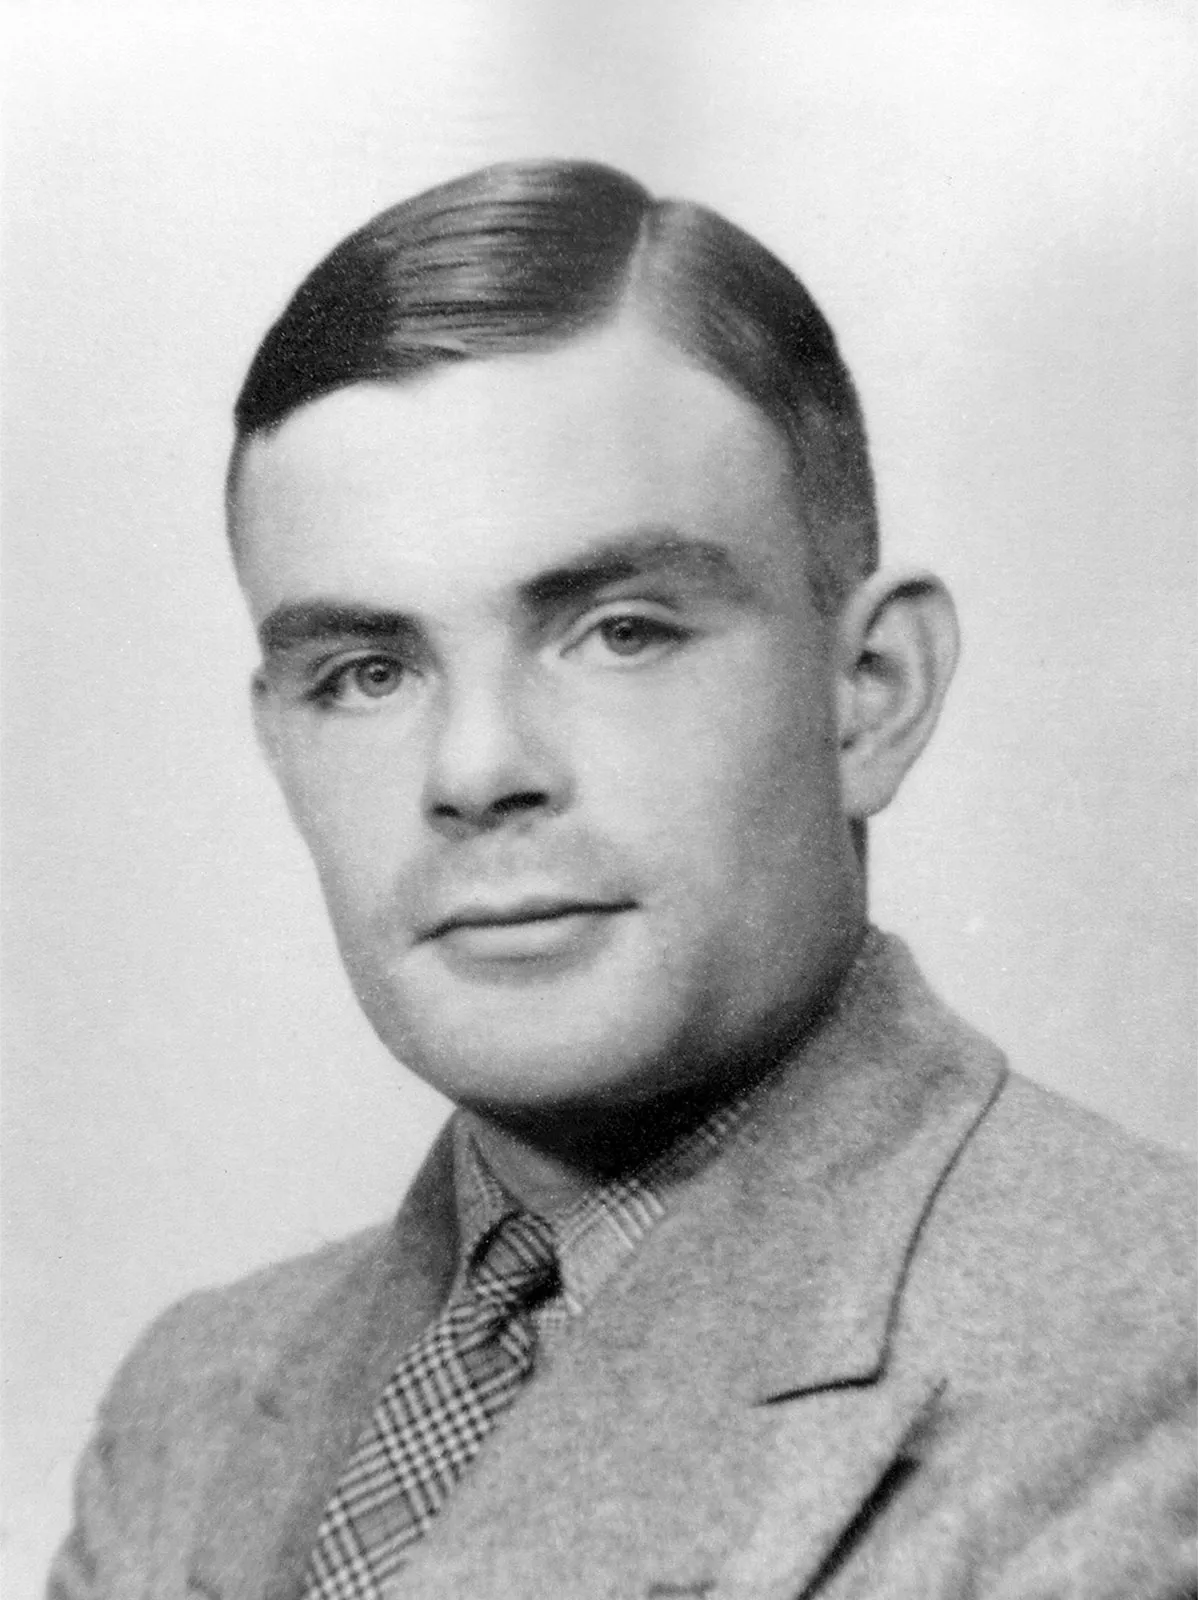
\includegraphics[scale=0.08]{Alan-Turing.png}
	\caption{Alan Turing}
	\label{obr1}
\end{figure}
\\\\
Alan Turing vo svojom výskume ohľadne umelej inteligencie nemohol pokračovať pretože výpočtová technika v období pred rokom 1950 nebola dostatočná pre jeho výskum pretože počítače vedeli príkazy len vykonávať, nemali žiadnu pamäť na zapamätanie si vykonaných príkazov. Ďalší problém boli vysoké náklady na prevádzkovanie a prenajímanie počítačov, čo si mohli dovoliť len prestížne univerzity a spoločnosti, nie individuálni výskumníci.\cite{HAI}
\begin{table}[tbh]
	\centering
	\caption{Porovnanie cien počítačov}
	\begin{tabular}{p{1.2in} p{1.3in} p{0.7in} p{1.1in}}
		1951 & 1965 & 1977 & 1982\\ \hline
		UNIVAC & IBM System/360 & Apple II & Commodore 64\\
		130 000\$/mesiac & 253 000\$ & 5800\$ & 1670\$\\
	\label{tab:cenyPC}
	\end{tabular}
\end{table}

V roku 1956 bol vytvorený prvý program ktorý používal skutočnú umelú inteligenciu s názvom Logic Theorist. Jeho tvorcovia boli Herbert Alexander Simon, Allen Newell a John Clifford Shaw. Tento program bol prvý ľudský vynález, ktorý vedel uvažovať na ľudskej úrovni. Podstatou tohto programu bolo riešenie rôznych matematických problémov a vyhotovenie matematických dôkazov, kde pri jednej z 52 teorém vyhotovil dôkaz detailnejšie ako pôvodní autori danej teorémy.      

\subsection{Prvé použitie umelej inteligencie vo videohrách} \label{kapitola2.1}
Umelá inteligencia vo videohrách bola prvý krát použítá vo videohre Nim, kde bolo cieľom poraziť súpera v odstraňovaní zápaliek z herného poľa. Herné poľe predstavuje 4 rady zápaliek a hra spočíva v tom, že hráč ktorý je na rade si zvolí ľubovoľný rad a odoberie z neho rôzne množstvo zápaliek. Hráč ktorý odoberie zápaľku alebo zápaľky ako posledný, vyhráva hru. 
\begin{figure}[tbh]
	\centering
	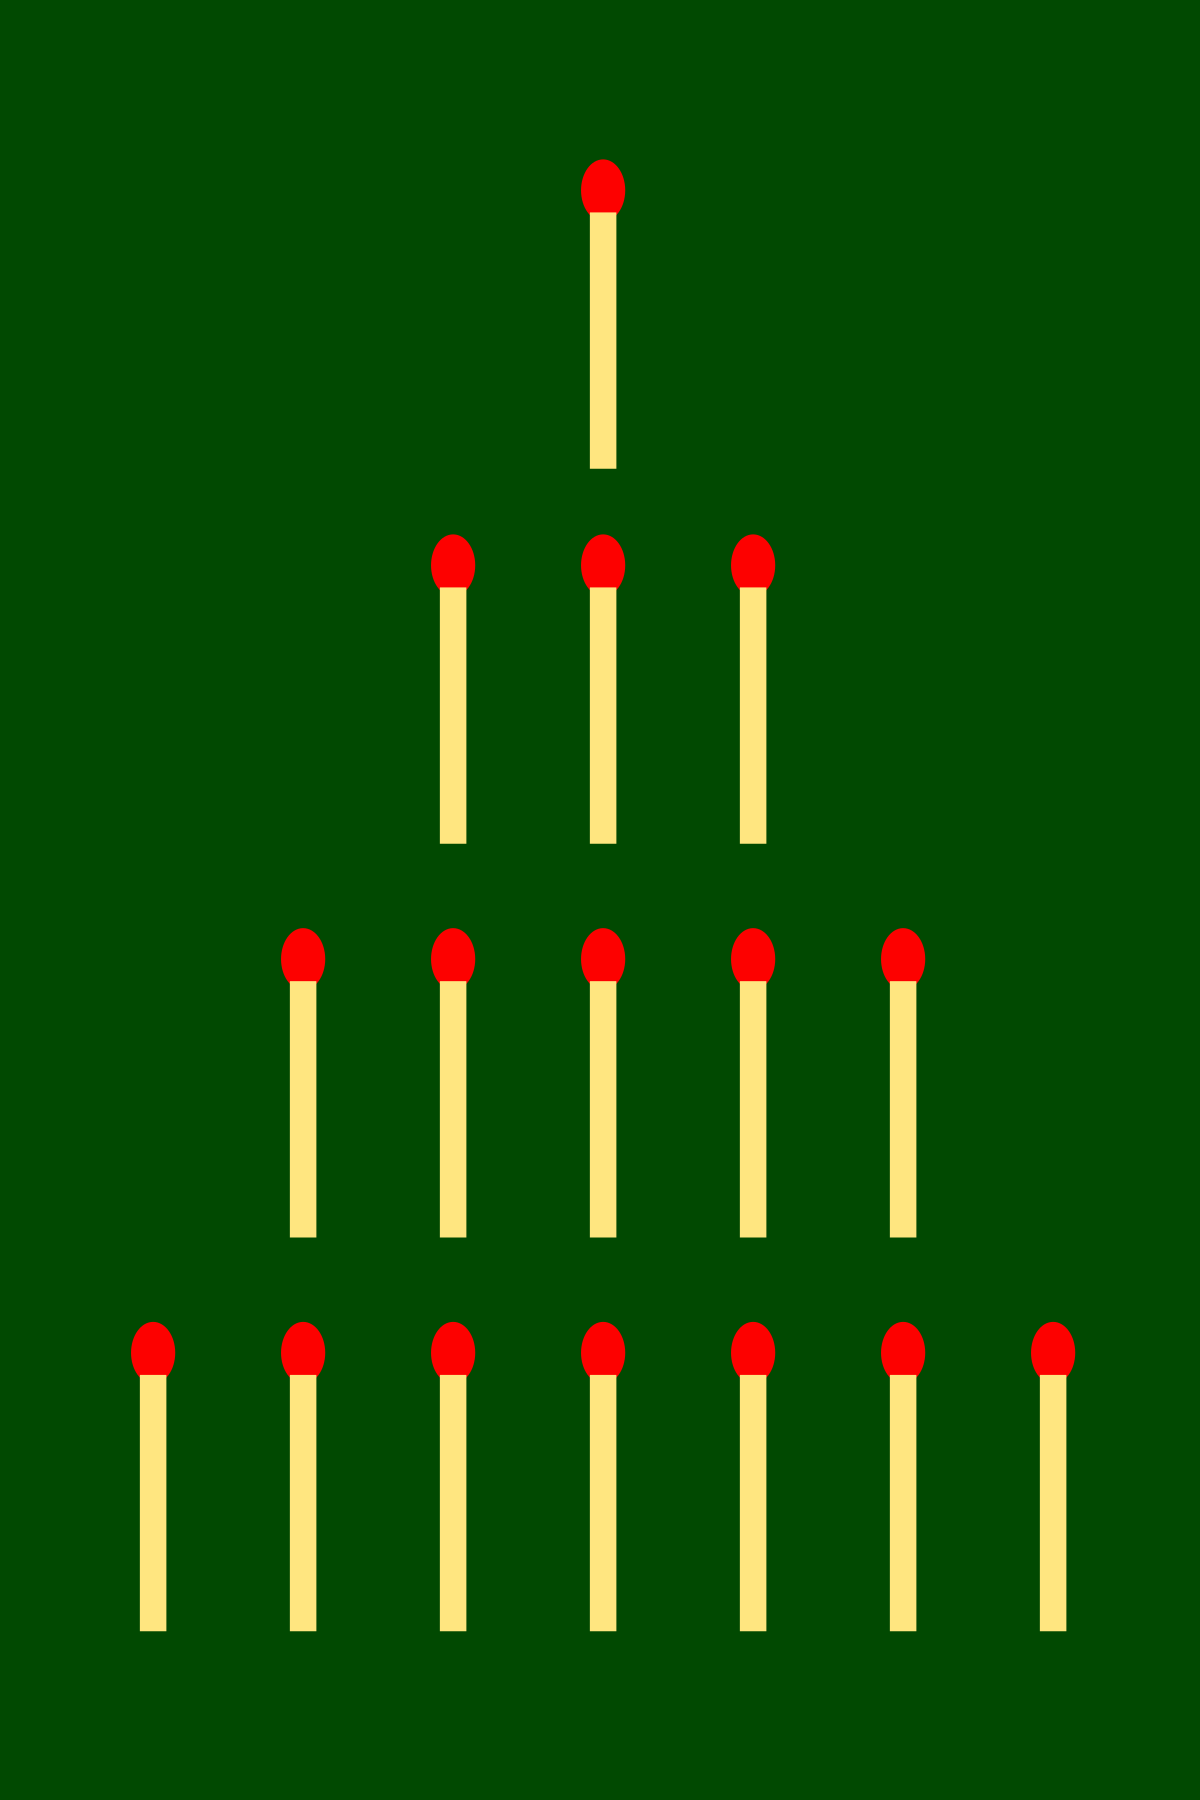
\includegraphics[scale=0.06]{NimGame.png}
	\caption{Videohra Nim}
	\label{obr2}
\end{figure}

\subsection{Videohry pred rokom 2000 používajúce umelú inteligenciu} \label{kapitola2.2}
Videohry sa začali vytvárať až po druhej svetovej vojne a počas studenej vojny pretože tieto udalosti pomohli vývoju výpočtovej techniky čo znamenalo, že viacej a viacej ľudí malo prístup k týmto technológiam čiže vývoj výpočtovej techniky sa začal zväčšovať exponenciálne. V roku 1980 bola vytvorená hra Pac-Man ktorá mala zakomponovanú už o niečo komplikovanejšiu umelú inteligenciu ako videohra Nim, ale stále to boli len jednoduché algoritmy. Vo videohre Pac-Man ale na rozdiel od hry Nim bola umelá inteligencia použitá 4 krát vo forme duchov ktorý počas hry prenásledujú hráča na základe 4 rozdielnych algoritmov. \cite{PacmanAI}

Červený duch prenásleduje hráča priamo, neuvažuje nad tým, akými možnými cestami môže hráč utiecť.

Ružový duch funguje veľmi podobne ako červený duch, ale odlišuje sa od prvého v tom, že nehľadá najkratšiu cestu k hráčovi, ale pred hráča.

Modrý duch sa správa tak, že ako prvé sa zoberie pozícia pred hráčom, rovnako ako pri ružovom duchovi, ďalej sa výtvorí úsečka medzi týmto bodom a červeným duchom. Úsečka sa otočí o 180 stupňov doprava a bod, ktorý bol na červenom duchovi je teraz cieľ modrého ducha, takže najkratšou možnou cestou sa k tomuto bodu snaží dostať a tento proces sa neustále vykonáva pre čo najväčšiu presnosť.

Oranžový duch funguje tak, že ak je viacej ako osem políčok ďaleko od hráča, tak funguje ako červený duch, ale ak je dostatočne blízko, tak mení svoj algoritmus a ide najkratšou možnou cestou do dolného ľavého rohu. Medzi týmito dvoma algoritmami neustálne prepína čím pôsobí na hráča nepredvídateľne čo je aj jeho úlohou, aby hráč spravil chybu a jeden z ďalších troch duchov ho chytil.
\begin{figure}[tbh]
	\centering
	
\includegraphics[scale=0.2]{redGhost.png}
	
\includegraphics[scale=0.2]{pinkGhost.png}
	
\includegraphics[scale=0.2]{blueGhost.png}
	
\includegraphics[scale=0.2]{orangeGhost.png}
	\caption{Pac-Man Duchovia}
	\label{obr3}
\end{figure}

\subsection{Umelá inteligencia v moderných videohrách} \label{kapitola2.3}
O 34 rokov vývoja umelej inteligencie neskôr, vyšla hra s názvom Alien Isolation v ktorej je umelá inteligencia zakomponovaná do nepriateľov, nazývaných votrelci. Týchto votrelcov riadia dve umelé inteligencie. \cite{AlienIsolationAI} Sú rozdelené tak, že jedna neustále vie, kde sa hráč nachádza ale tá druhá o tom nevie. Cieľom tej prvej inteligencie je navádzať tú druhú tak, aby vedela na čo sa má sústrediť, napríklad keď votrelec naposledy videl hráča utiecť do miestnosti, kde sa dá schovať do rôznych objektov, tak tá inteligencia, ktorá vie kde sa nachádza hráč povie tej druhej, nech skontroluje tieto objekty. Pomimo umelej inteligencie má tento votrelec v sebe zakomponované aj meradlo, čím meria intenzitu stresu ktorú hráč prežíva, tým, že vidí votrelca alebo je v jeho blízkosti a ak sa toto meradlo naplní, tak prvá inteligencia prikazuje tej druhej, aby išla preč od hráča čím si hráč môže nachvíľu oddychnúť. Toto striedanie medzi útekom od votrelca a schovávaním pred ním udržuje hráča hrať túto hru a neodradí ho po prvej hodine alebo dvoch hrania. Ako bolo spomenuté, druhá umelá inteligencia votrelca nikdy nevie presne kde sa hráč nachádza, len na základe poskytnutých informácií prvou umelou inteligenciou postupuje podľa naprogramovaného stromového grafu v ktorom sa nachádza cez 100 možností na výber. Niektoré tieto možnosti sa ale odomknú až po dosiahnutí určitých úrovní kvôli tomu, aby sa votrelec po danom čase hrania nezdal opakujúci.


\section{Algoritmy umelej inteligencie} \label{kapitola3}
Umelá inteligencia sú v podstate algoritmy, ktoré sa snažia napodobniť to, ako sa má daná inteligentná forma života správať. Najčastejšie používané algoritmy v umelej inteligencii vo videohrách je algoritmus hľadania cesty a algoritmus rozhodovania sa.

\subsection{Algoritmus hľadania cesty} \label{kapitola3.1}
Z anglického slova “path finding”, tento algoritmus je jeden z najpoužívanejších v moderných videohrách pretože je veľmi flexibilný, čo vývojári hier veľmi obľubujú. Jeho cieľom je nájsť najkratšiu cestu z bodu A do bodu B. 

\subsection{Algoritmus rozhodovania sa} \label{kapitola3.2}
Tento algoritmus určuje, čo a na základe akých okolností vykoná umelá inteligencia. Vstupom sú dáta z okolia, kde sa umelá inteligencia nachádza a z týchto vstupov usudzuje, čo má spraviť ďalej. Ako taký príklad môže byť, že hráč strieľa po umelej inteligencii ktorá na základe tohto vstupu, sa rozhodne, že sa skryje za najbližšiu prekážku a začne opätovať streľbu.


\section{Typy umelej inteligencie} \label{kapitola4}
Umelá inteligencia vo videohrách v porovnaní s tou v iných odvetiach sa odlišuje v tom, že tá v hrách je vytvorená väčšinou tak, aby napodobňovala inú inteligentnú formu života. Kvôli tomuto nikdy nedosiahne svôj úplný potenciál a je nútená v mnohých prípadoch byť porazená hráčom. Napríklad v spomenutej hre Pac-Man \ref{kapitola2.2}, každý duch má špeciálne vytvorenú umelú inteligenciu tak, aby hráč mal šancu vyhrať danú úroveň a kvôli tomuto je táto hra zábavná. Umelá inteligencia mimo hier, ktorými sú napríklad virtuálny asistent Alexa alebo Google Assistant ktorého nájdeme v dnešnej dobe v mnohých moderných zariadeniach ako sú naše smartfóny alebo tablety ale aj smart televízie, používajú strojové učenie (Machine Learning) čo je vlastne podkategóriou umelej inteligencie a pomáha jej zlepšovať sa v ich práci bez vypisovania veľkého počtu riadkov inštrukcií. Táto vlastnosť je veľmi dôležitá a užitočná, pretože týto asistenti nepracujú s presne vytýčenými vstupmi pretože každý človek je iný, napríklad človek 1 povie virtuálnemu asistentovi aby mu nastavil upozornenie na zasadnutie inak ako by to povedal človek 2, buď sa odlišujú v nárečí, použitím slov alebo rôznymi inými spôsobmi. Jednoducho, umelá inteligencia v hrách sa najčastejšie riadi podľa presne vytýčených algoritmov pretože počet vstupov, ktoré hráč môže zadať je limitovaný na rozdiel od tej využívanej mimo hier, ktorá tiež používa nejaké algoritmy ale hlavným rozdielom je použitie strojového učenia, skoro neobmedzeného množstva vstupov a umožnenie dovŕšenia úplného potenciálu, nakoľko nie je limitovaná imitáciou nejakej inteligentnej formy života ako vo videohrách.


\section{Záver} \label{zaver} % prípadne iný variant názvu



%\acknowledgement{Ak niekomu chcete poďakovať\ldots}


% týmto sa generuje zoznam literatúry z obsahu súboru literatura.bib podľa toho, na čo sa v článku odkazujete
\bibliography{literatura}
\bibliographystyle{plain} % prípadne alpha, abbrv alebo hociktorý iný
\end{document}
